\PassOptionsToPackage{unicode=true}{hyperref} % options for packages loaded elsewhere
\PassOptionsToPackage{hyphens}{url}
%
\documentclass[ignorenonframetext,]{beamer}
\usepackage{pgfpages}
\setbeamertemplate{caption}[numbered]
\setbeamertemplate{caption label separator}{: }
\setbeamercolor{caption name}{fg=normal text.fg}
\beamertemplatenavigationsymbolsempty
% Prevent slide breaks in the middle of a paragraph:
\widowpenalties 1 10000
\raggedbottom
\setbeamertemplate{part page}{
\centering
\begin{beamercolorbox}[sep=16pt,center]{part title}
  \usebeamerfont{part title}\insertpart\par
\end{beamercolorbox}
}
\setbeamertemplate{section page}{
\centering
\begin{beamercolorbox}[sep=12pt,center]{part title}
  \usebeamerfont{section title}\insertsection\par
\end{beamercolorbox}
}
\setbeamertemplate{subsection page}{
\centering
\begin{beamercolorbox}[sep=8pt,center]{part title}
  \usebeamerfont{subsection title}\insertsubsection\par
\end{beamercolorbox}
}
\AtBeginPart{
  \frame{\partpage}
}
\AtBeginSection{
  \ifbibliography
  \else
    \frame{\sectionpage}
  \fi
}
\AtBeginSubsection{
  \frame{\subsectionpage}
}
\usepackage{lmodern}
\usepackage{amssymb,amsmath}
\usepackage{ifxetex,ifluatex}
\usepackage{fixltx2e} % provides \textsubscript
\ifnum 0\ifxetex 1\fi\ifluatex 1\fi=0 % if pdftex
  \usepackage[T1]{fontenc}
  \usepackage[utf8]{inputenc}
  \usepackage{textcomp} % provides euro and other symbols
\else % if luatex or xelatex
  \usepackage{unicode-math}
  \defaultfontfeatures{Ligatures=TeX,Scale=MatchLowercase}
\fi
% use upquote if available, for straight quotes in verbatim environments
\IfFileExists{upquote.sty}{\usepackage{upquote}}{}
% use microtype if available
\IfFileExists{microtype.sty}{%
\usepackage[]{microtype}
\UseMicrotypeSet[protrusion]{basicmath} % disable protrusion for tt fonts
}{}
\IfFileExists{parskip.sty}{%
\usepackage{parskip}
}{% else
\setlength{\parindent}{0pt}
\setlength{\parskip}{6pt plus 2pt minus 1pt}
}
\usepackage{hyperref}
\hypersetup{
            pdftitle={Docker in Action: Second Edition},
            pdfauthor={Chapter 04},
            pdfborder={0 0 0},
            breaklinks=true}
\urlstyle{same}  % don't use monospace font for urls
\newif\ifbibliography
\usepackage{graphicx,grffile}
\makeatletter
\def\maxwidth{\ifdim\Gin@nat@width>\linewidth\linewidth\else\Gin@nat@width\fi}
\def\maxheight{\ifdim\Gin@nat@height>\textheight\textheight\else\Gin@nat@height\fi}
\makeatother
% Scale images if necessary, so that they will not overflow the page
% margins by default, and it is still possible to overwrite the defaults
% using explicit options in \includegraphics[width, height, ...]{}
\setkeys{Gin}{width=\maxwidth,height=\maxheight,keepaspectratio}
\setlength{\emergencystretch}{3em}  % prevent overfull lines
\providecommand{\tightlist}{%
  \setlength{\itemsep}{0pt}\setlength{\parskip}{0pt}}
\setcounter{secnumdepth}{0}

% set default figure placement to htbp
\makeatletter
\def\fps@figure{htbp}
\makeatother


\title{Docker in Action: Second Edition}
\author{Chapter 04}
\date{Working with storage and volumes}

\begin{document}
\frame{\titlepage}

\hypertarget{working-with-storage-and-volumes}{%
\section{Working with storage and
volumes}\label{working-with-storage-and-volumes}}

\begin{frame}{Text Book}
\protect\hypertarget{text-book}{}

\begin{figure}
\centering
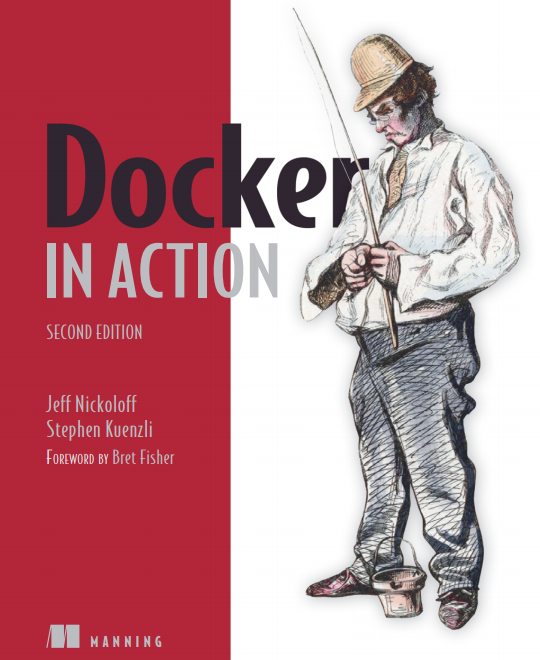
\includegraphics[width=\textwidth,height=3.64583in]{./tex2pdf.-d218b5bed17bed47/9157dca3b5e68de9ca71f68394cbf91d05a2314a.png}
\caption{\emph{itmt 495/595 textbook}}
\end{figure}

\end{frame}

\begin{frame}{Chapter 04 - Objectives}
\protect\hypertarget{chapter-04---objectives}{}

\begin{itemize}
\tightlist
\item
  Demonstrate mount points
\item
  Demonstrate how to share data between the host and a container
\item
  Demonstrate how to share data between containers
\item
  Explain the concept of using temporary, in-memory filesystems
\item
  Explain how to managing data with volumes
\item
  Discuss advanced storage with volume plugins
\end{itemize}

\end{frame}

\begin{frame}{Concept Review}
\protect\hypertarget{concept-review}{}

\begin{itemize}
\tightlist
\item
  From chapter 01:

  \begin{itemize}
  \tightlist
  \item
    What are the two Linux concepts/features that make up a Linux
    Container?
  \item
    Docker was created in what year/month?
  \item
    Is the focus of Docker containers infrastructure or application
    deployment?
  \item
    What is a Docker Container image?
  \item
    What is a Docker Container instance?
  \item
    What is the difference between a Linux Container and a Virtual
    Machine?
  \end{itemize}
\end{itemize}

\end{frame}

\begin{frame}[fragile]{Concept Review 2}
\protect\hypertarget{concept-review-2}{}

\begin{itemize}
\tightlist
\item
  What is \texttt{-\/-detached} mode?
\item
  What is a CID?
\item
  What does it mean to link two containers?
\end{itemize}

\end{frame}

\begin{frame}[fragile]{Concept Review 3}
\protect\hypertarget{concept-review-3}{}

\begin{itemize}
\tightlist
\item
  What are the three methods for obtaining Docker Images?
\item
  What is a registry?
\item
  Is a Docker Image a file?
\item
  What is a layer?
\item
  What is a major advantage of filesystem layers in Docker?
\item
  How does the use of namespaces and \texttt{chroot} allow for
  filesystems to work in Docker?
\end{itemize}

\end{frame}

\begin{frame}{Introduction}
\protect\hypertarget{introduction}{}

\begin{itemize}
\tightlist
\item
  So far we have run a bunch of containers

  \begin{itemize}
  \tightlist
  \item
    They have been trivial applications
  \end{itemize}
\item
  What if we want to run a real application?
\item
  What if we had a database?

  \begin{itemize}
  \tightlist
  \item
    Where would that file be stored?
  \item
    Is it in a file inside the container?
  \item
    What happens to that data when you stop the container or remove the
    container?
  \item
    Where would you write log files so that they will outlive the
    container?
  \item
    How would you get access to those logs to troubleshoot a problem?
  \item
    How can other programs such as log digest tools get access to those
    files?
  \end{itemize}
\end{itemize}

\end{frame}

\begin{frame}{File trees and mount points - 4.1}
\protect\hypertarget{file-trees-and-mount-points---4.1}{}

\begin{figure}
\centering
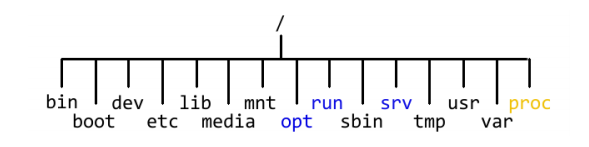
\includegraphics{./tex2pdf.-d218b5bed17bed47/4bca1da672e7a55d4ea76c418b0dd551142883e3.png}
\caption{\emph{Linux Filesystem}}
\end{figure}

\begin{itemize}
\tightlist
\item
  Storage devices such as disk partitions or USB disk partitions are
  attached to specific locations in that tree
\item
  Those locations are called \textbf{mount points}
\item
  A mount point defines the location in the tree

  \begin{itemize}
  \tightlist
  \item
    The access properties to the data at that point (for example,
    writability)
  \item
    The source of the data mounted at that point (for example, a
    specific hard disk, USB device, or memory-backed virtual disk)
  \end{itemize}
\end{itemize}

\end{frame}

\begin{frame}{Mounts}
\protect\hypertarget{mounts}{}

\begin{itemize}
\tightlist
\item
  Mount points allow software and users to use the file tree in a Linux
  environment

  \begin{itemize}
  \tightlist
  \item
    Without knowing exactly how that tree is mapped into specific
    storage devices
  \end{itemize}
\item
  Logic follows that if different storage devices can be mounted at
  various points in a file tree, we can mount nonimage-related storage
  at other points in a container file tree
\item
  That is exactly how containers get access to storage on the host
  filesystem and share storage between containers
\item
  The best place to start is by understanding the three most common
  types of storage mounted into containers:

  \begin{itemize}
  \tightlist
  \item
    Bind mounts
  \item
    In-memory storage
  \item
    Docker volumes
  \end{itemize}
\end{itemize}

\end{frame}

\begin{frame}[fragile]{Storage Types}
\protect\hypertarget{storage-types}{}

\begin{itemize}
\tightlist
\item
  These storage types can be used in many ways\ldots{}

  \begin{itemize}
  \tightlist
  \item
    Figure 4.2 shows an example of a container filesystem
  \item
    That starts with the files from the image
  \item
    Adds an in-memory tmpfs at \texttt{/tmp}
  \item
    bind-mounts a configuration file from the host
  \item
    writes logs into a Docker volume on the host
  \end{itemize}
\end{itemize}

\begin{figure}
\centering
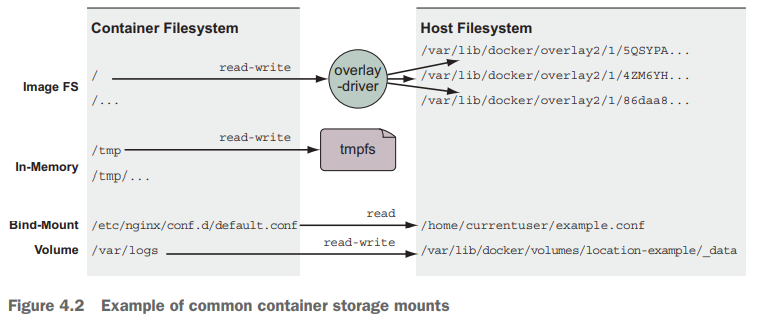
\includegraphics{./tex2pdf.-d218b5bed17bed47/cd97a05bfb8fd7d5b9ad2db9ae9c2a165575b964.png}
\caption{\emph{Figure4-2}}
\end{figure}

\end{frame}

\begin{frame}{Bind mounts - 4.2}
\protect\hypertarget{bind-mounts---4.2}{}

\begin{itemize}
\tightlist
\item
  Bind mounts are mount points used to remount parts of a filesystem
  tree onto other locations

  \begin{itemize}
  \tightlist
  \item
    Suppose you're running a web server that depends on sensitive
    configuration on the host and emits access logs that need to be
    forwarded by your log-shipping system
  \item
    You could use Docker to launch the web server in a container
  \item
    Then bind-mount the configuration location as well as the location
    where you want the web server to write log
  \item
    In Figure 4.3, lets deploy a web server container
  \item
    Let us deploy an log forwarder software container (theoretical)
  \item
    Let us demonstrate how mounts work and how we can share a single
    file between two containers
  \end{itemize}
\end{itemize}

\end{frame}

\begin{frame}{Figure 4.3}
\protect\hypertarget{figure-4.3}{}

\begin{figure}
\centering
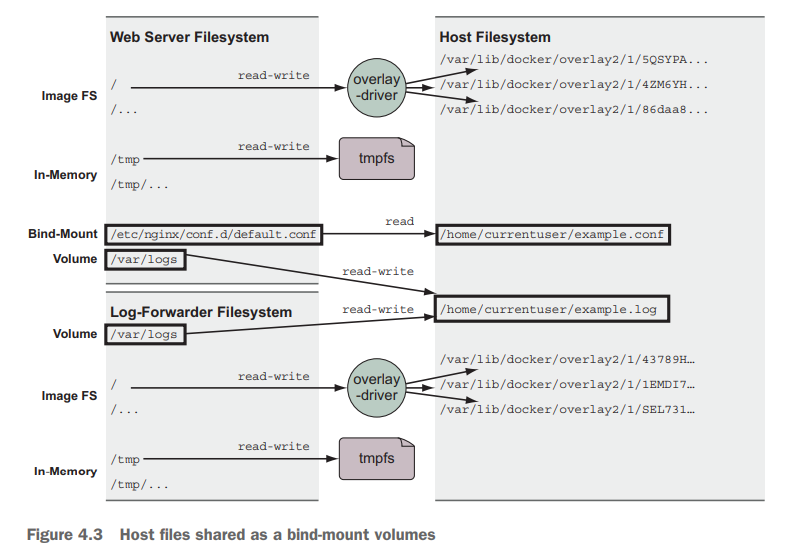
\includegraphics{./tex2pdf.-d218b5bed17bed47/b91c6062cd754d14e9e2e48bb29d473be7819b94.png}
\caption{\emph{Figure 4.3}}
\end{figure}

\end{frame}

\begin{frame}{Mount and Bind Options}
\protect\hypertarget{mount-and-bind-options}{}

\begin{itemize}
\tightlist
\item
  Lets look at printed page 65, 66, and 67

  \begin{itemize}
  \tightlist
  \item
    The main thing to capture here is that we are going to mount files
    from our local filesystem into the Docker Container
  \item
    Then we will set those conf files as read-only (for security)
  \item
    We will also enable the container to write a log file back to our
    local filesystem from the container
  \item
    But bind mounts are not optimal for general computing (say hosting a
    database file)
  \end{itemize}
\end{itemize}

\end{frame}

\begin{frame}{In-memory storage - 4.3}
\protect\hypertarget{in-memory-storage---4.3}{}

\begin{itemize}
\tightlist
\item
  Where to store secret or sensitive information?

  \begin{itemize}
  \tightlist
  \item
    Why not in-memory?
  \item
    Set the type option on the mount flag to tmpfs
  \item
    This is the easiest way to mount a memory-based filesystem into a
    container's file tree
  \item
    You can set quotas on this in-memory filesystem
  \end{itemize}
\end{itemize}

\end{frame}

\begin{frame}{Sample of in-memory}
\protect\hypertarget{sample-of-in-memory}{}

docker run --rm\\
--mount type=tmpfs,dst=/tmp\\
--entrypoint mount\\
alpine:latest -v

docker run --rm\\
--mount type=tmpfs,dst=/tmp,tmpfs-size=16k,tmpfs-mode=1770\\
--entrypoint mount\\
alpine:latest -v

\end{frame}

\begin{frame}[fragile]{Docker volumes - 4.3}
\protect\hypertarget{docker-volumes---4.3}{}

\begin{itemize}
\tightlist
\item
  In VirtualBox we have virtual harddrives or sometimes called `volumes'

  \begin{itemize}
  \tightlist
  \item
    This is not that
  \end{itemize}
\item
  Docker volumes are named filesystem trees managed by Docker

  \begin{itemize}
  \tightlist
  \item
    All operations on Docker volumes can be accomplished using the
    docker volume subcommand set
  \item
    \texttt{docker\ volume\ create}
  \item
    \texttt{docker\ volume\ inspect}
  \end{itemize}
\item
  Let us look at some examples in 4.4.1
\end{itemize}

\end{frame}

\begin{frame}{Summary - Part 1 of 2}
\protect\hypertarget{summary---part-1-of-2}{}

\begin{itemize}
\tightlist
\item
  This chapter covered mount points in depth, including the following:

  \begin{itemize}
  \tightlist
  \item
    Mount points allow many filesystems from many devices to be attached
    to a single file tree. Every container has its own file tree
  \item
    Containers can use bind mounts to attach parts of the host
    filesystem into a container
  \item
    In-memory filesystems can be attached to a container file tree so
    that sensitive or temporary data is not written to disk
  \item
    Docker provides anonymous or named storage references called volumes
  \end{itemize}
\end{itemize}

\end{frame}

\begin{frame}{Summary - Part 2 of 2}
\protect\hypertarget{summary---part-2-of-2}{}

\begin{itemize}
\tightlist
\item
  Volumes can be created, listed, and deleted using the appropriate
  docker volume subcommand
\item
  Volumes are parts of the host filesystem that Docker mounts into
  containers at specified locations
\item
  Volumes have life cycles of their own and might need to be
  periodically cleaned up
\item
  Docker can provide volumes backed by network storage or other more
  sophisticated tools if the appropriate volume plugin is installed
\end{itemize}

\end{frame}

\begin{frame}{Deliverable}
\protect\hypertarget{deliverable}{}

\begin{itemize}
\tightlist
\item
  Using the Nginx Docker image \url{https://hub.docker.com/_/nginx}

  \begin{itemize}
  \tightlist
  \item
    Create an Nginx load balancer
  \item
    Use a volume mount to mount the necessary configuration files into
    the container and mount as ro
  \item
    Add a tmpfs mount
  \item
    Create 3 additional Nginx webserver to display hello world sample
    code provided

    \begin{itemize}
    \tightlist
    \item
      In the jhajek repo under itmt-495-595: container-lb-sample
    \end{itemize}
  \end{itemize}
\end{itemize}

\end{frame}

\begin{frame}{Questions}
\protect\hypertarget{questions}{}

Any questions?

\end{frame}

\end{document}
